%
% This is the LaTeX template file for lecture notes for EE 382C/EE 361C.
%
% To familiarize yourself with this template, the body contains
% some examples of its use.  Look them over.  Then you can
% run LaTeX on this file.  After you have LaTeXed this file then
% you can look over the result either by printing it out with
% dvips or using xdvi.
%
% This template is based on the template for Prof. Sinclair's CS 270.

\documentclass[twoside]{article}
\usepackage{graphicx}
\usepackage{wrapfig}
\usepackage{amsmath}
\usepackage{amssymb}
\usepackage{listings}
\usepackage{float}
\usepackage{capt-of}
\usepackage{pifont}
\setlength{\oddsidemargin}{0.25 in}
\setlength{\evensidemargin}{-0.25 in}
\setlength{\topmargin}{-0.6 in}
\setlength{\textwidth}{6.5 in}
\setlength{\textheight}{8.5 in}
\setlength{\headsep}{0.75 in}
\setlength{\parindent}{0 in}
\setlength{\parskip}{0.1 in}

%
% The following commands set up the lecnum (lecture number)
% counter and make various numbering schemes work relative
% to the lecture number.
%
\newcounter{lecnum}
\renewcommand{\thepage}{\thelecnum-\arabic{page}}
\renewcommand{\thesection}{\thelecnum.\arabic{section}}
\renewcommand{\theequation}{\thelecnum.\arabic{equation}}
\renewcommand{\thefigure}{\thelecnum.\arabic{figure}}
\renewcommand{\thetable}{\thelecnum.\arabic{table}}

%
% The following macro is used to generate the header.
%
\lstset{language=Python, numbers=left, tabsize=2, xleftmargin=5.0ex,breaklines=true,}

\newcommand{\lecture}[4]{
   \pagestyle{myheadings}
   \thispagestyle{plain}
   \newpage
   \setcounter{lecnum}{#1}
   \setcounter{page}{1}
   \noindent
   \begin{center}
   \framebox{
      \vbox{\vspace{2mm}
    \hbox to 6.28in { {\bf EE 382V: Parallel Algorithms
                        \hfill Summer 2017} }
       \vspace{4mm}
       \hbox to 6.28in { {\Large \hfill Lecture #1: #2  \hfill} }
       \vspace{2mm}
       \hbox to 6.28in { {\it Lecturer: #3 \hfill Scribe: #4} }
      \vspace{2mm}}
   }
   \end{center}
   \markboth{Lecture #1: #2}{Lecture #1: #2}
   %{\bf Disclaimer}: {\it These notes have not been subjected to the
   %usual scrutiny reserved for formal publications.  They may be distributed
   %outside this class only with the permission of the Instructor.}
   \vspace*{4mm}
}

%
% Convention for citations is authors' initials followed by the year.
% For example, to cite a paper by Leighton and Maggs you would type
% \cite{LM89}, and to cite a paper by Strassen you would type \cite{S69}.
% (To avoid bibliography problems, for now we redefine the \cite command.)
% Also commands that create a suitable format for the reference list.
\renewcommand{\cite}[1]{[#1]}
\def\beginrefs{\begin{list}%
        {[\arabic{equation}]}{\usecounter{equation}
         \setlength{\leftmargin}{2.0truecm}\setlength{\labelsep}{0.4truecm}%
         \setlength{\labelwidth}{1.6truecm}}}
\def\endrefs{\end{list}}
\def\bibentry#1{\item[\hbox{[#1]}]}

%Use this command for a figure; it puts a figure in wherever you want it.
%usage: \fig{NUMBER}{SPACE-IN-INCHES}{CAPTION}
\newcommand{\fig}[3]{
			\vspace{#2}
			\begin{center}
			Figure \thelecnum.#1:~#3
			\end{center}
	}
% Use these for theorems, lemmas, proofs, etc.
\newtheorem{theorem}{Theorem}[lecnum]
\newtheorem{lemma}[theorem]{Lemma}
\newtheorem{proposition}[theorem]{Proposition}
\newtheorem{claim}[theorem]{Claim}
\newtheorem{corollary}[theorem]{Corollary}
\newtheorem{definition}[theorem]{Definition}
\newenvironment{proof}{{\bf Proof:}}{\hfill\rule{2mm}{2mm}}

% **** IF YOU WANT TO DEFINE ADDITIONAL MACROS FOR YOURSELF, PUT THEM HERE:

\begin{document}
%FILL IN THE RIGHT INFO.
%\lecture{**LECTURE-NUMBER**}{**DATE**}{**LECTURER**}{**SCRIBE**}
\lecture{7}{June 16}{Vijay Garg}{Ari Bruck}
%\footnotetext{These notes are partially based on those of Nigel Mansell.}

% **** YOUR NOTES GO HERE:

% Some general latex examples and examples making use of the
% macros follow.  
%**** IN GENERAL, BE BRIEF. LONG SCRIBE NOTES, NO MATTER HOW WELL WRITTEN,
%**** ARE NEVER READ BY ANYBODY.
\section{Introduction}
During this lecture, we continued our discussion of parallel implementation of algorithms. We were exposed again to the benefits of cascading algorithms as well as Parallel Prefix to reach work optimal algorithms. The topics covered in class include:
\begin{itemize}
	\item The \texttt{merge} Algorithm
	\item Dijkstra's Guarded Command Language
	\item The \texttt{rank} Operation
	\item List Ranking (Pointer Jumping)
\end{itemize}

This set of lecture notes will briefly re-examine the topics covered in this lecture, in the order in which they appeared during class.

\section{The \texttt{merge} Algorithm}
When we discussed \texttt{merge} in class, we are specifically referring to the merging of two sorted arrays of size=\texttt{n} into an array of size=\texttt{2*n}.

The professor then asked us to write a sequential algorithm for merging two arrays. A proposed solution was the following:
\begin{lstlisting}
i,j,k = 0,0,0;
while (i < n and j <n) {
	if (A[i] < B[j]) { C[k] = A[i]; i++;} 
	else             { C[k] = A[j]; j++;}
	k++;
}
while (i<n) {
	C[k] = A[i];
	i++; k++;
}
while (j<n) {
	C[k] = A[j];
	j++; k++;
}
\end{lstlisting}
$T(n) = O(n)$

$W(n) = O(n)$

\subsection{Dijkstra's Guarded Command Language}
We were introduced to Dijkstra's Guarded Command Language in relation to the sequential merge algorithm. 
For example, the if statement inside the while loop in the above code would be re-written to:

\begin{lstlisting}
[ // <- guarded statement
	(A[i] <= B[j]) C[k] := A[i]; i++; k++;
	(B[j] <= A[i]) C[k] := B[j]; j++; k++;
]
\end{lstlisting}
If both guards are equivalent and true then the program is non-deterministic. This is not necessarily a bad thing!

\section{The \texttt{scatter} Operation}
Here were recapped the terminology used in parallel algorithms. There are
\begin{itemize}
	\item \texttt{reduce}
	\item \texttt{scan}
	\item \texttt{scatter} // this is new
\end{itemize}

To merge, we pick a random element in array $A$ and see where it goes into C.

$Rank(A[i],C)$ = $(i-1)$ number of elements in $A$ less than $A[i]$ + $rank(A[i],B)$.

The reason we sort is to do search easy i.e. binary search in $O(\log(n))$ time.
\textbf{So the overall time is:}

$T(n) = O(1) + O(\log(n))$

This requires concurrent read but no concurrent write so a $CREW$ PRAM. However this is not work optimal since it requires $n$ processors doing $O(\log(n))$ work, or:

$W(n) = O(n * \log(n))$

So how do we improve this? Use cascading!

\begin{figure}[h]
\center
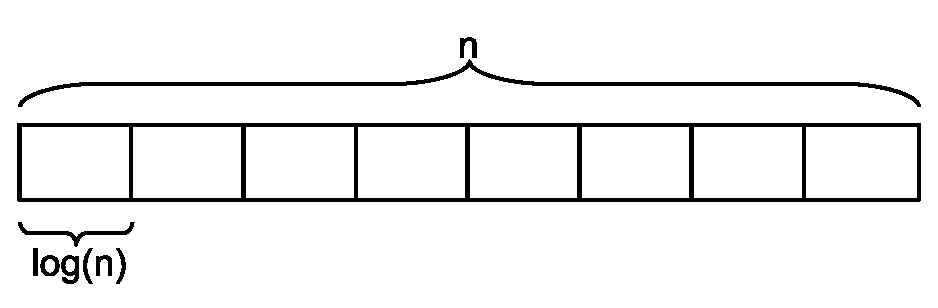
\includegraphics[scale=0.5]{img/cascade_split.eps}
\end{figure}

Think of each element at first block. Call these splitters. 

The number of splitters = $O(n/\log(n))$

Merge the splitters: $T(n)=O(n)$
\begin{figure}[H]
\center
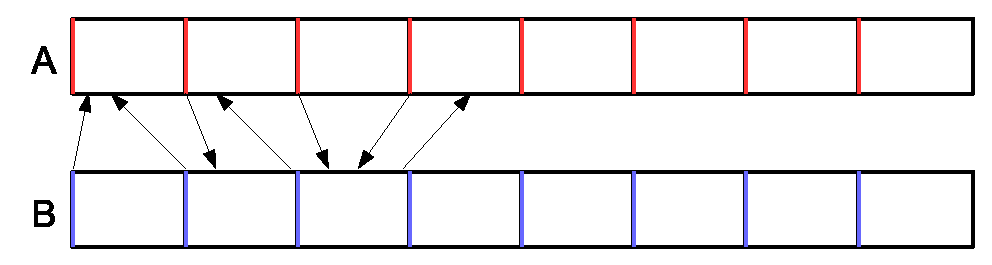
\includegraphics[scale=0.5]{img/merge.eps}
\caption{The splitters could go anywhere but the key is they can never cross. A crossing line indicates it was smaller in A but no bigger in B). We can order it in $O(\log(n))$.}
\end{figure}

The algorithm would look like:
\begin{enumerate}
    \item Break array into splitters and non-splitters
    \item Merge all splitters: $O(n/\log(n)) * O\log(n)) = O(n)$ work in $T(n) = O(\log(n))$
    \item Apply sequential algorithm to small segment to merge non-splitters in parallel: $T(n) = O(\log(n))$, $W(n) = O(n)$
\end{enumerate}
\textbf{Overall:}

$T(n) = O(\log(n))$

$W(n) = O(n)$ so this is work optimal

\section{List Ranking}
\textbf{Goal:} Find the distance from the tail of linked-list.

\begin{figure}[h]
\center
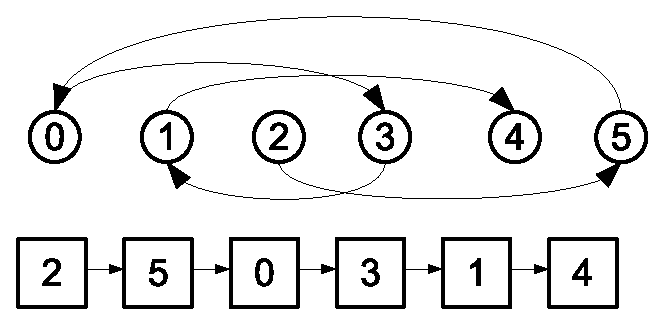
\includegraphics[scale=0.5]{img/linked_list.eps}
\end{figure}

In finding the parallel implementation, first write down the sequential algorithm to find the work-optimal solution.

\textbf{Sequential Algorithm:}

Iterate through all elements until the tail is reached.

$T(n)=O(n)$

$W(n)=O(n)$

\textbf{Parallel Algorithm:}\textit{We are looking for} $T(n)=\log(n)$

Let's get closer to god/nirvana! We will add another pointer that points to grandparent. This reduces everybody by 2 since grandparent also pointed to their grandparent. 

\begin{figure}[H]
\center
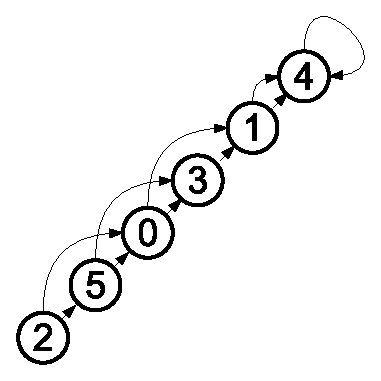
\includegraphics[scale=0.5]{img/pointer_jumping.eps}
\caption{This is called \textbf{Pointer Jumping}}
\end{figure}
The reduction by 2 is the log(n) we are looking for:
$T(n)=O(\log(n))$

\subsection{Pointer Jumping Algorithm} 

\textbf{Input:} Given to you for every \texttt{i}, \texttt{next[i]}.

\begin{lstlisting}
for all i in parallel do:
    Q[i] := next[i] // make a copy of next[]

for all i in parallel do:
    if (Q[i]==-1) then R[i] := 0 // If this is the tail
    else          then R[i] := 1

for all i in parallel do:
    while ((Q[i] != -1) && (Q[Q[i]] != -1)) do // if parent and grandparent exists
        Q[i] := Q[Q[i]]
        R[i] := R[i] + R[Q[Q[i]]]
    end while
\end{lstlisting}
\textit{This is for a $PRAM$, for a GPU there needs to be a barrier so everyone is in sync}

\subsection{Pointer Jumping Example}
Let's work through an example that will show us the algorithm.

\begin{center}
\begin{table}[h]
\center
\begin{tabular}{ |c|c|c|c|c|c|c| } 
 \hline
 \textbf{Array:} & 2 & 5 & 0 & 3 & 1 & 4 \\
 \hline
 \texttt{i:} & 0 & 1 & 2 & 3 & 4 & 5 \\ 
 \texttt{Next:} & 3 & 4 & 5 & 1 & -1 & 0 \\ 
 \texttt{Q:} & 3 & 4 & 5 & 1 & -1 & 0 \\ 
 \texttt{R:} & 1 & 1 & 1 & 1 & 0 & 1 \\ 
 \hline
\end{tabular}
\caption{Simulation at time T=0}
\end{table}
\end{center}


\begin{table}[H]
    \begin{minipage}[H]{.5\textwidth }
        \footnotesize
        \begin{tabular}{ |c|c|c|c|c|c|c| } 
 \hline
 \textbf{Array:} & 2 & 5 & 0 & 3 & 1 & 4 \\
 \hline
 \texttt{i:} & 0 & 1 & 2 & 3 & 4 & 5 \\ 
 \texttt{Q:} & 1 & 4 & 0 & 4 & -1 & 3 \\ 
 \texttt{R:} & 2 & 1 & 2 & 2 & 0 & 2 \\ 
 \hline
        \end{tabular}
        \caption{Simulation at time T=1}
    \end{minipage}%
    \begin{minipage}[H]{.5\textwidth}
        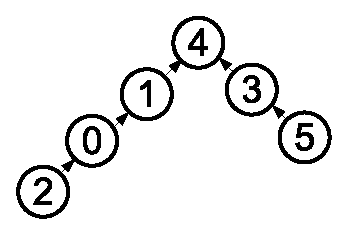
\includegraphics[width=0.45\textwidth, scale=0.5]{img/iter_1.eps}
        \captionof{figure}{Linked list as a tree after 1 iteration}
    \end{minipage}
\end{table}

\begin{table}[H]
    \begin{minipage}[H]{.5\textwidth }
        \footnotesize
        \begin{tabular}{ |c|c|c|c|c|c|c| } 
 \hline
 \textbf{Array:} & 2 & 5 & 0 & 3 & 1 & 4 \\
 \hline
 \texttt{i:} & 0 & 1 & 2 & 3 & 4 & 5 \\ 
 \texttt{Q:} & 4 & 4 & 1 & 4 & -1 & 4 \\ 
 \texttt{R:} & 3 & 1 & 4 & 2 & 0 & 4 \\ 
 \hline
        \end{tabular}
        \caption{Simulation at time T=2}
    \end{minipage}%
    \begin{minipage}[H]{.5\textwidth}
        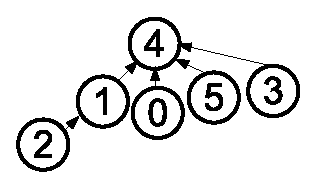
\includegraphics[width=0.45\textwidth, scale=0.5]{img/iter_2.eps}
        \captionof{figure}{Linked list as a tree after 2 iterations - at every iteration we are compressing the height}
    \end{minipage}
\end{table}

\begin{table}[H]
    \begin{minipage}[H]{.5\textwidth }
        \footnotesize
        \begin{tabular}{ |c|c|c|c|c|c|c| } 
 \hline
 \textbf{Array:} & 2 & 5 & 0 & 3 & 1 & 4 \\
 \hline
 \texttt{i:} & 0 & 1 & 2 & 3 & 4 & 5 \\ 
 \texttt{Q:} & 4 & 4 & 4 & 4 & -1 & 4 \\ 
 \texttt{R:} & 3 & 1 & 5 & 2 & 0 & 4 \\ 
 \hline
        \end{tabular}
        \caption{Simulation at time T=3}
    \end{minipage}%
    \begin{minipage}[H]{.5\textwidth}
        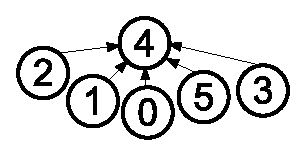
\includegraphics[width=0.45\textwidth, scale=0.5]{img/iter_3.eps}
        \captionof{figure}{Linked list as a tree after 3 iterations}
    \end{minipage}
\end{table}

This algorithm takes $O(\log(n))$ time where n is the size of the linked list. It does $O(n * \log(n))$ work and is therefore not work-optimal.

\subsection{Work-Optimal Pointer-Jumping}
Let's see if parallel prefix can help us. In the past implementations, we jumped by even entries:
\begin{enumerate}
    \item Divide array into even nodes/entries and odd entries
    \item Only the even entries do the work (compute parallel prefix recursively)
    \item Odd entries in parallel use the even's parallel prefix answers to compute theirs
\end{enumerate}

\textit{Q:} So how do we do this? In an array it was easy to choose the odd and even entries. This is not so in a linked list.

\textit{A:} Use a randomizer (coin flip). Each element will flip a coin to decide whether that element will be chosen. To do this effectively we will set some rules for choosing elements:
\begin{itemize}
    \item two consecutive nodes cannot be chosen
    \item two dots are not too much apart (in order to do the sequential algorithm efficiently)
\end{itemize}

\textbf{\underline{Independent Set:}} In a graph, nodes that do not share an edge are independent.

Everybody flip a coin to get Tail or Heads. Node chooses itself if they get heads and their \texttt{Next} is tails.

Probability guarantees that the time until \texttt{Next} is soon (probability increases 1/2 every turn). Expected distance between chosen node is $O(1)$.

P(node is not chosen) = 3/4

\begin{table}[H]
    \center
    \begin{tabular}{ |c|c|c| } 
        \hline
        \textbf{My Flip} & \textbf{My \texttt{Next}'s flip} & \textbf{Chosen} \\
        \hline
        H & H & \ding{55} \\ 
        H & T & \ding{51} \\ 
        T & H & \ding{55} \\ 
        T & T & \ding{55} \\
        \hline
    \end{tabular}
    
    \caption{Choosing of element in linked list given its and its neighbor's flip Truth table}
\end{table}

Recursively move to next level to then reduce to 1. The list is shrunken by constant fraction so therefore in expected $O(\log(n))$ iterations, the list is shrunk to 1.

\textbf{Overall:}

$T(n) = O(\log(n))$

$W(n) = O(n)$

\end{document}